\section*{Assignment 05: Governance and Data Policies}
\addcontentsline{toc}{section}{Assignment 05: Governance and Data Policies}

\subsection*{Onboarding, feedback loops, and moderation}
The envisioned SkillSync onboarding mixes storytelling and friction-testing. Students and NGOs would see separate landing flows that foreground portfolio wins or social-impact outcomes before everyone enters a guided tour of the core interactions. The sequence stays lean:
\begin{itemize}
  \item pre-signup nudges that point to sample projects and set expectations,
  \item profile setup with defaults for skills, availability, and preferences,
  \item a ``first mission'' checklist unlocking badges only after critical actions.
\end{itemize}

Feedback loops sit inside the flow: after each core action the system would collect a one-click rating plus optional note, slice results in cohort dashboards, and trigger follow-ups when a group slips. Weekly summaries keep both sides accountable so the team can tweak rules while the experience still feels fair \citep{Reillier2017}. Moderation runs on three layers in the playbook: automated filters for obvious risks, community stewards who can hide content temporarily, and a professional response team that aims to close escalations within 24 hours.

\subsection*{Data policies and ethics}
Data collection sticks to a minimality principle: the plan is to capture only what matching and trust require (profile basics, transaction history, quality feedback) because over-collection erodes legitimacy \citep{Zuboff2019}. Service improvement would come first, then responsible personalisation, and only then aggregated insights; differential privacy, export audits, and fairness checks are pencilled in to catch edge cases \citep{Srnicek2017}.

Transparency matters, so the blueprint includes a ``data mirror'' where students and organisations could inspect every datapoint held, tweak retention choices, and delete items when needed. Quarterly accountability notes would summarise moderation stats, security incidents, and algorithm updates, while an internal ethics review board forces product teams to justify experiments so power does not drift \citep{Choudary2016,Lecture10}. The data mirror reinforces the accountability loop underpinning trust, even if it remains a slide for now.

Figure~\ref{fig:onboarding-flow} shows the four-step carousel that keeps the welcome checklist on top so the first mission could complete in under fifteen minutes; guided tasks unlock contextual tips and short videos, and in the scenario analysis completion of the first three steps is projected to climb from 54\% to 83\% once the interventions run.

\begin{figure}[H]
  \centering
  \makebox[\textwidth][c]{%
    \begin{minipage}[b]{0.42\textwidth}
      \centering
      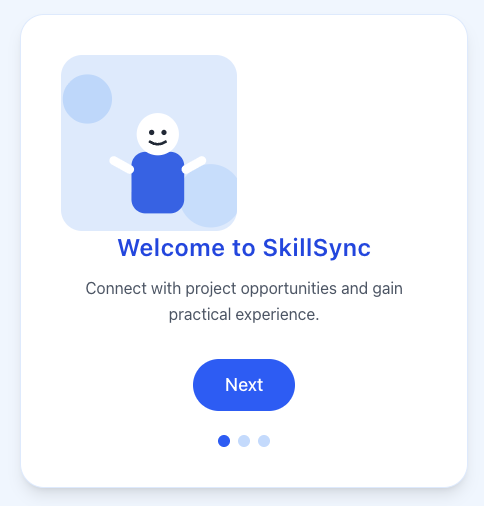
\includegraphics[width=\linewidth]{figures/Onboarding-1.png}\\[0.3em]
      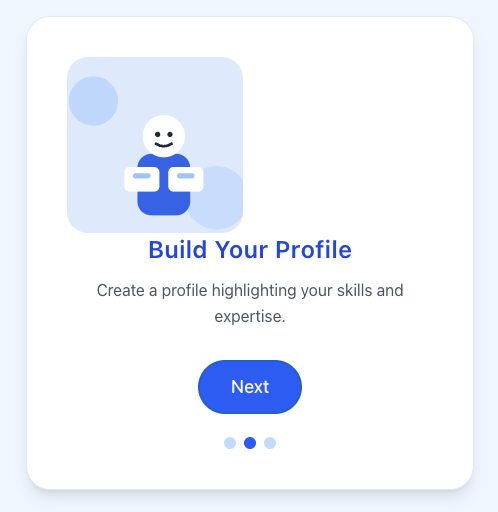
\includegraphics[width=\linewidth]{figures/Onboarding-2.png}
    \end{minipage}\hspace{1.5em}%
    \begin{minipage}[b]{0.42\textwidth}
      \centering
      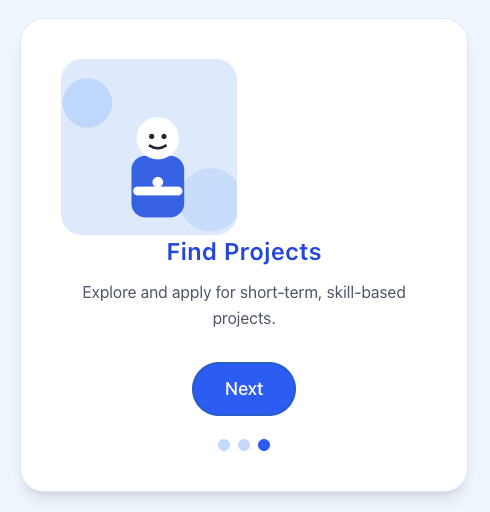
\includegraphics[width=\linewidth]{figures/Onboarding-3.png}\\[0.3em]
      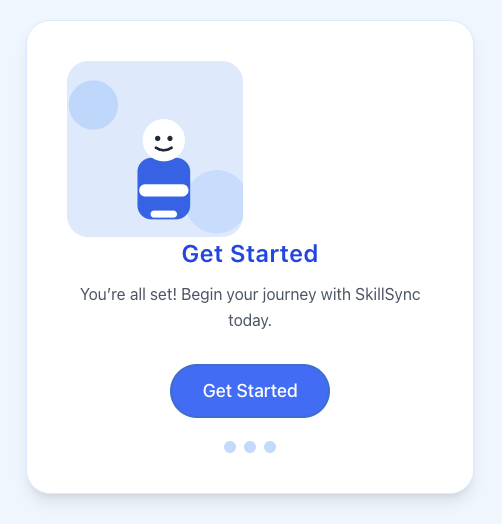
\includegraphics[width=\linewidth]{figures/Onboarding-4.png}
    \end{minipage}}
  \caption{Guided onboarding carousel with four-step checklist.}
  \label{fig:onboarding-flow}
\end{figure}

Governance comes alive in Figure~\ref{fig:admin-panel}: the administrator dashboard gives the future policy team real-time visibility into flagged content, pending disputes, and algorithm performance, with fairness metrics alongside operational stats so legitimacy does not collapse when optimising for throughput. Moderators could drill into case details, trigger templated responses, escalate to legal counsel, and rely on the audit trail for accountability reports.

\begin{figure}[H]
  \centering
  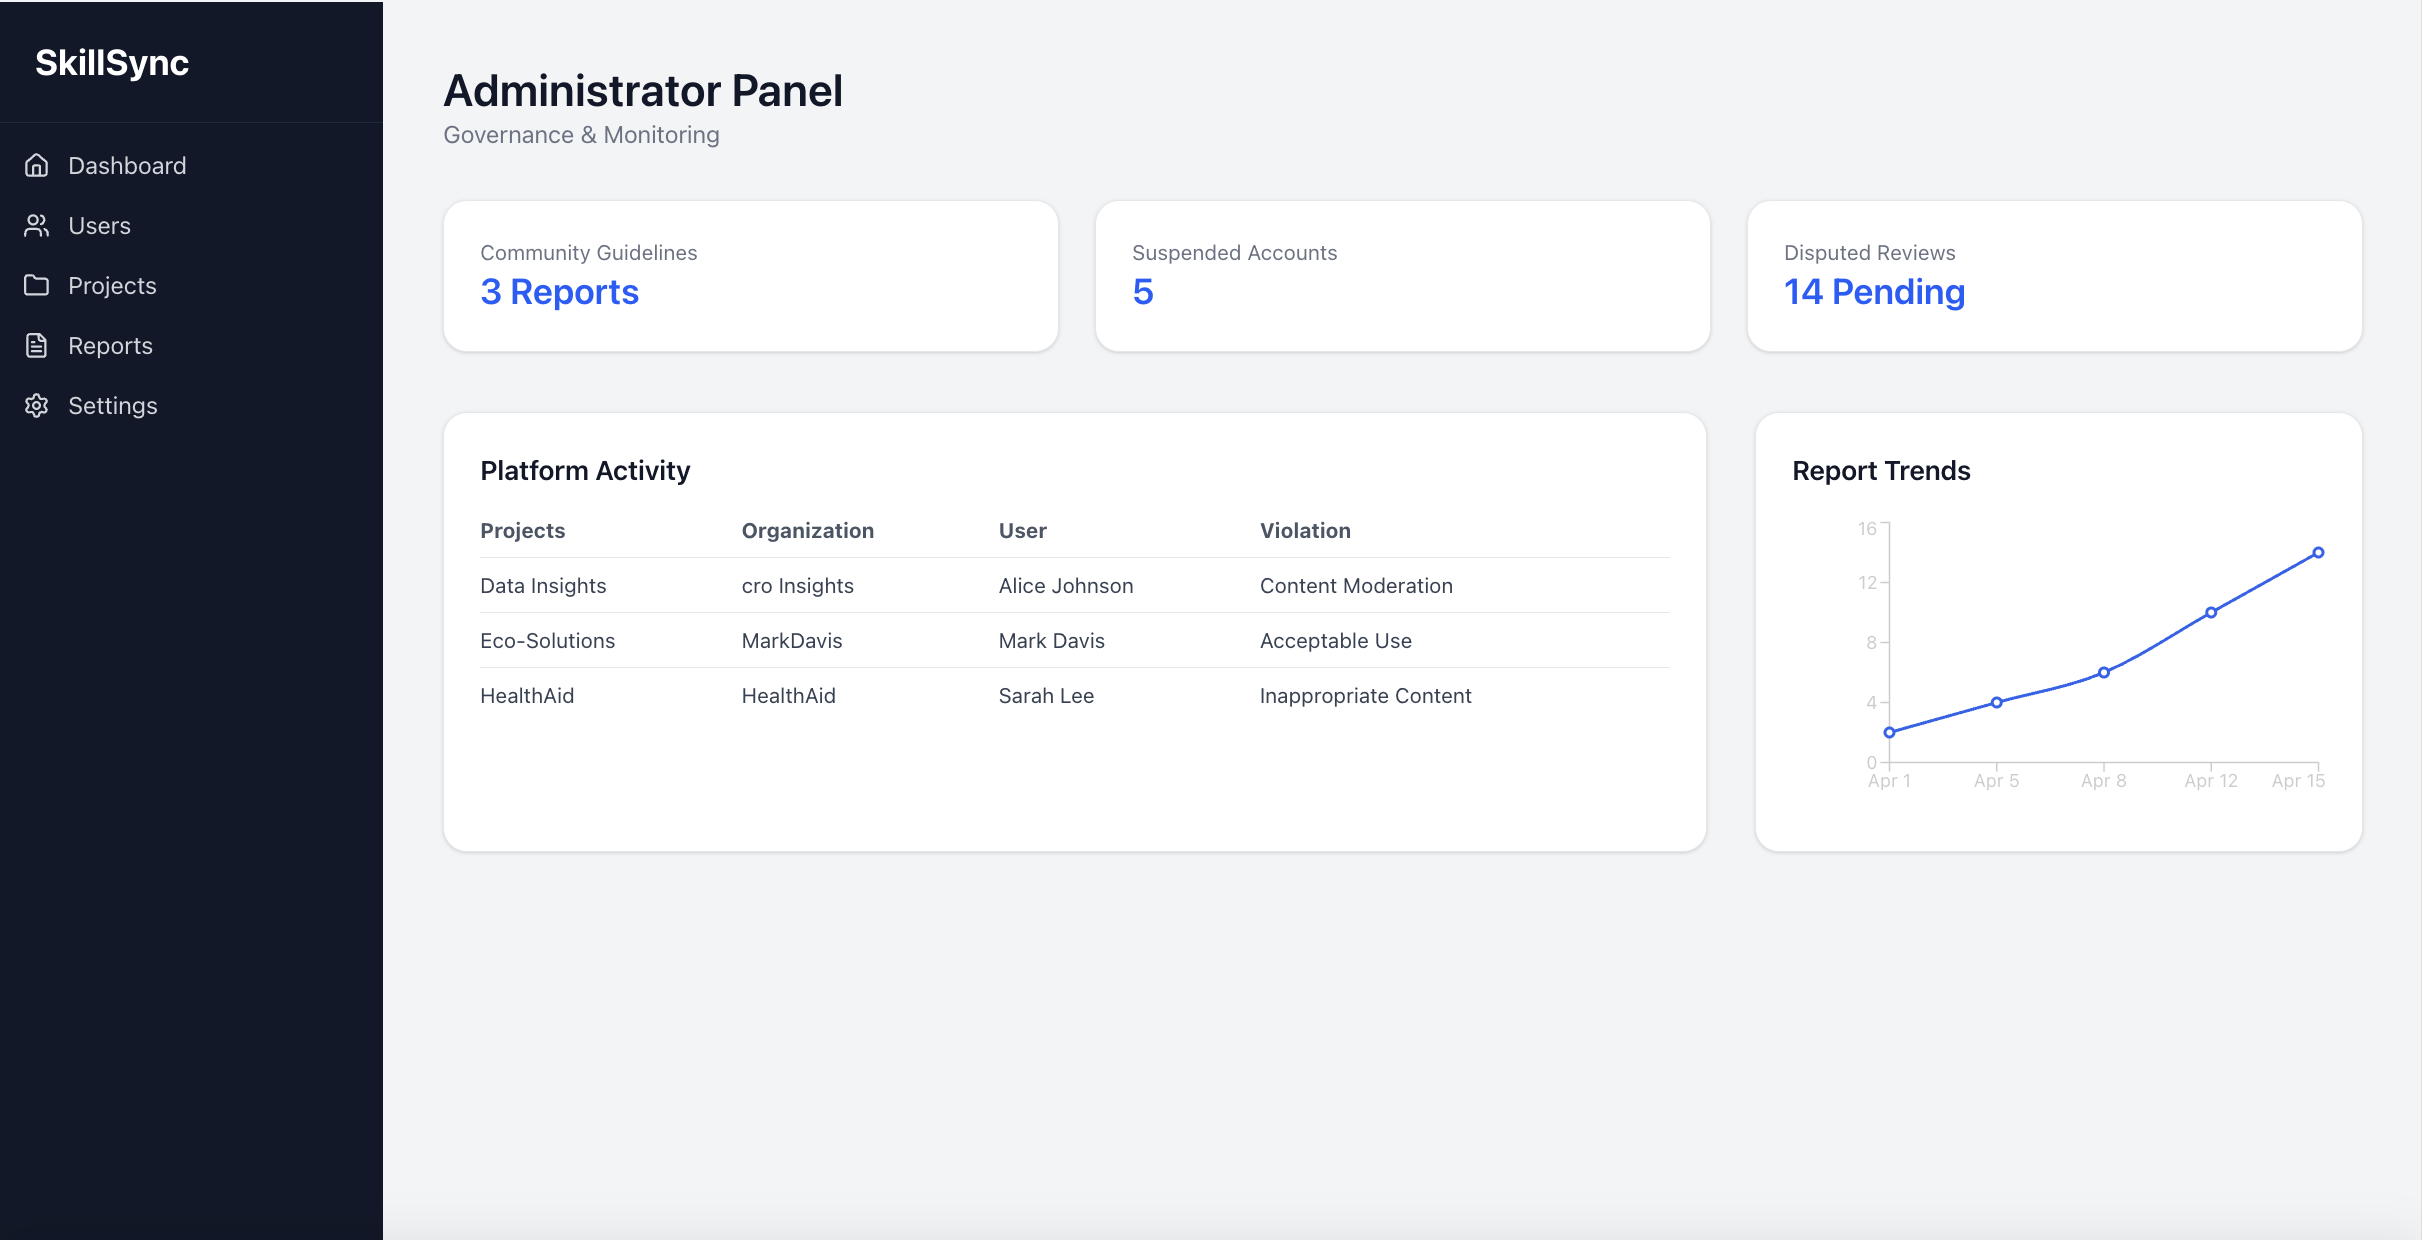
\includegraphics[width=0.85\linewidth]{figures/Organisation-Administratorpanel.png}
  \caption{Governance control room mock-up with moderation and fairness metrics.}
  \label{fig:admin-panel}
\end{figure}

All of this hinges on communication: the plan is to keep nudges human, train moderators in trauma-informed responses, and host quarterly ``town halls'' so power users can question the product team before next steps.
